\documentclass{beamer}

\usetheme{Madrid}
\usepackage[utf8]{inputenc}
\usepackage[T1]{fontenc}
\usepackage[francais]{babel}
\usepackage{amsmath}
\usepackage{multirow}
\usepackage{textpos}
\usepackage{minted}

% Get rid of the navigation bars
\beamertemplatenavigationsymbolsempty
% Change itemization markers to 'squares'
\useinnertheme{rectangles}
\setbeamertemplate{itemize items}[triangle]

\author[DePierre]{Tao "DePierre" S.}
\title{Buffer overflow}
\institute[HackGyver]{
\includegraphics[height=3cm,width=3cm]{images/LogoHackGyver.png}\\\large{Le hackerspace de Belfort}}
\date{8 mai 2013}
\logo{
\includegraphics[height=1.5cm,width=1.5cm]{images/LogoHackGyver.png}}

\begin{document}

% Title page
\begin{frame}[plain]
	\maketitle
\end{frame}

% Table of contents
\begin{frame}{Plan}
	\tableofcontents
\end{frame}

% Options for the display of the table of contents
\AtBeginSubsection[]
{
   \begin{frame}
        \frametitle{Buffer overflow}
        \tableofcontents[ 
    		currentsubsection, 
    		currentsubsections, 
    	] 
   \end{frame}
}

\section{Définition}

\begin{frame}{Définition formelle}
	\begin{center}
		"In computer security and programming, a buffer overflow, or buffer overrun, is an anomaly where a program, while writing data to a buffer, overruns the buffer's boundary and overwrites adjacent memory." (Wikipedia)
	\end{center}
\end{frame}

\section{En mémoire}
\subsection{Vue générale}

\begin{frame}{Vue générale}
	\begin{center}
		\begin{tabular}{| c |}
    		\hline
   			\\
    		Text\\ 
    		\\ \hline
    		\\
    		(Initialized)\\
    			Data\\
    		(Uninitialized)\\
    		\\ \hline
    		\\
    		Stack\\
    		\\
    		\hline
		\end{tabular}
		$\downarrow$ memory addresses
	\end{center}
\end{frame}

\begin{frame}{Fonctionnement de la stack}
	\begin{center}
		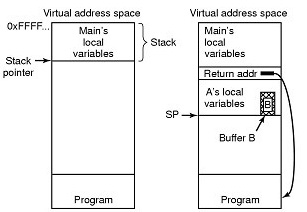
\includegraphics[width=0.8\textwidth]{images/stack.jpg}
	\end{center}
\end{frame}

\subsection{Etude de la stack}

\begin{frame}[fragile]{Exemple 1 (1/3)}
	\definecolor{bg}{rgb}{0.95,0.95,0.95}
	\begin{minted}[mathescape,
               linenos,
               numbersep=5pt,
               frame=lines,
               framesep=2mm,
               bgcolor=bg,
               baselinestretch=0.3,
               fontize=\footnotesize]{c}
void function(int a, int b, int c) {
    char buffer[20];
}

int main(int argv, char *argc[]) {
    function(1, 2, 3);
    return 0;
}
	\end{minted}
\end{frame}

\begin{frame}[fragile]{Exemple 1 (2/3)}
	La fonction 'main'
	\definecolor{bg}{rgb}{0.95,0.95,0.95}
	\begin{minted}[mathescape,
               linenos,
               numbersep=5pt,
               frame=lines,
               framesep=2mm,
               bgcolor=bg,
               baselinestretch=0.3,
               fontize=\footnotesize]{nasm}
push   ebp
mov    ebp,esp
sub    esp,0xc
mov    DWORD PTR [esp+0x8],0x3
mov    DWORD PTR [esp+0x4],0x2
mov    DWORD PTR [esp],0x1
call   0x80483d0 <function>
mov    eax,0x0
leave  
ret
	\end{minted}
\end{frame}

\begin{frame}[fragile]{Exemple 1 (3/3)}
	La fonction 'function'
	\definecolor{bg}{rgb}{0.95,0.95,0.95}
	\begin{minted}[mathescape,
               linenos,
               numbersep=5pt,
               frame=lines,
               framesep=2mm,
               bgcolor=bg,
               baselinestretch=0.3,
               fontize=\footnotesize]{nasm}
push   ebp ; Push the frame pointer onto the stack
mov    ebp,esp ; EBP now contains the new frame pointer
sub    esp,0x20 ; Allocate space for the local variables
leave  
ret
	\end{minted}
\end{frame}

\begin{frame}[fragile]{Exemple 2}
	La nouvelle fonction 'function'
	\definecolor{bg}{rgb}{0.95,0.95,0.95}
	\begin{minted}[mathescape,
               linenos,
               numbersep=5pt,
               frame=lines,
               framesep=2mm,
               bgcolor=bg,
               baselinestretch=0.3,
               fontize=\footnotesize]{c}
void function() {
    int i = 0;
    int tabint[20] = {0};
    for (i = 0; i < 20; i = i + 1)
        tabint[i] = i;
}
	\end{minted}
	L'état de la stack après son exécution
	\begin{minted}[mathescape,
               linenos,
               numbersep=5pt,
               frame=lines,
               framesep=2mm,
               bgcolor=bg,
               baselinestretch=0.3,
               fontize=\footnotesize]{objdump}
0xffffd8d8:	0x00000001	0x00000002	0x00000003	0x00000004
0xffffd8e8:	0x00000005	0x00000006	0x00000007	0x00000008
0xffffd8f8:	0x00000009	0x0000000a	0x0000000b	0x0000000c
0xffffd908:	0x0000000d	0x0000000e	0x0000000f	0x00000010
0xffffd918:	0x00000011	0x00000012	0x00000013	0x00000014
	\end{minted}
\end{frame}

\subsection{Récapitulatif}

\begin{frame}{Avec la stack}
	\begin{itemize}
		\itemsep1.3em
		\item On sait
		\begin{itemize}
			\itemsep1.3em
			\item comment l'espace est alloué
			\item comment sont stockés les valeurs
		\end{itemize}
		\item Plus on copie, plus on monte dans les adresses
	\end{itemize}
\end{frame}

\begin{frame}{Résumé}
	\begin{center}
		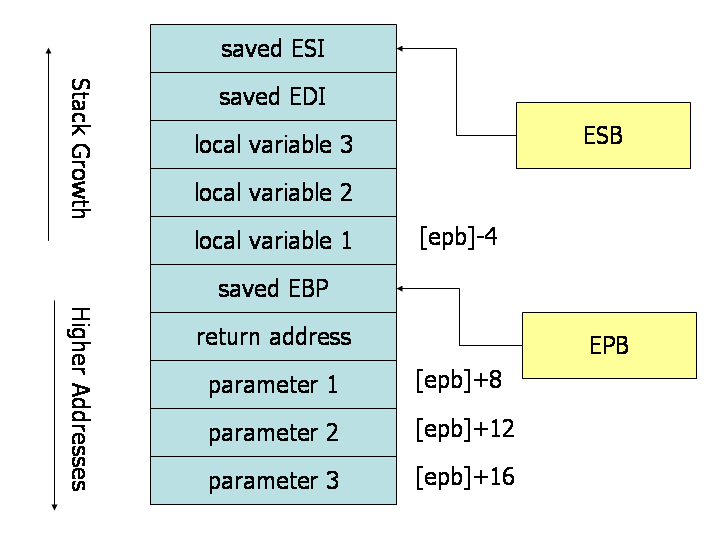
\includegraphics[width=0.8\textwidth]{images/stack-convention.png}
	\end{center}
\end{frame}

\begin{frame}{Justement !}
	\begin{center}
		\Large Que se passe-t-il si on continue de copier ?
	\end{center}
\end{frame}

\section{Smash the stack}
\subsection{Stratégie}

\begin{frame}{Stratégie}
	\begin{itemize}
		\itemsep1.3em
		\item Plus on écrit, plus les adresses \Large{$\nearrow$}
		\item L'adresse de retour se trouve plus loin
		\item Donc, si on dépasse, on \textbf{écrasera} l'adresse de retour
	\end{itemize}
	\begin{center}
		\Large $\Rightarrow$Contrôle du flux d'exécution!
	\end{center}
\end{frame}

\begin{frame}{Dépasser le buffer}
	\begin{center}
		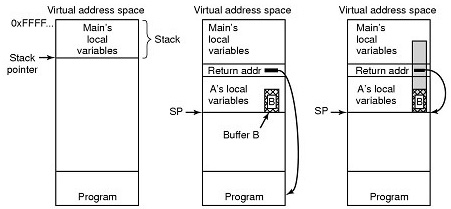
\includegraphics[width=1\textwidth]{images/buffer_overflow_attack.jpg}
	\end{center}
\end{frame}

\subsection{Méthode}

\begin{frame}{Smash the Stack}
	\begin{enumerate}
		\itemsep1.3em
		\item Trouver le buffer overflow
		\item Stocker notre shellcode
		\begin{itemize}
			\item Directement dans le buffer
			\item Dans une variable d'environnement
		\end{itemize}
		\item Ecraser l'adresse de retour
		\begin{itemize}
			\item Avec l'adresse du buffer
			\item Avec l'adresse de la variable d'env.
		\end{itemize}
		\item Poursuivre l'exécution
		\item Enjoy \Large{\textbackslash o/}
	\end{enumerate}
\end{frame}

\begin{frame}{Shellcode}
	\begin{center}
		"In computer security, a shellcode is a small piece of code used as the payload in the exploitation of a software vulnerability. It is called "shellcode" because it typically starts a command shell from which the attacker can control the compromised machine. [..] Shellcode is commonly written in machine code." (Wikipedia)
	\end{center}
\end{frame}

\begin{frame}{Shellcode}
	\begin{itemize}
		\itemsep1.3em
		\item[] Pour faire simple
		\begin{itemize}
			\itemsep1.3em
			\item Code machine
			\item Lance /bin/bash
			\item Ne peut pas contenir de NUL BYTE (0x00)
		\end{itemize}
		\item[] Exemple :
		\begin{itemize}
			\item[] \textbackslash x31\textbackslash xc0\textbackslash x50\textbackslash x68\textbackslash x2f\textbackslash x2f\textbackslash x73\textbackslash x68\textbackslash x68\textbackslash x2f\textbackslash x62\textbackslash x69\textbackslash x6e\\ \textbackslash x89\textbackslash xe3\textbackslash x50 \textbackslash x89\textbackslash xe2\textbackslash x53\textbackslash x89\textbackslash xe1\textbackslash xb0\textbackslash x0b\textbackslash xcd\textbackslash x80
		\end{itemize}
		\item[] (La création d'un shellcode n'est pas abordée ici)
	\end{itemize}
\end{frame}

\begin{frame}{Contenu de notre buffer}
	\begin{itemize}
		\itemsep1.3em
		\item Contient le shellcode (25 bytes avec l'exemple d'avant)
		\item Contient l'adresse qui pointe sur le début du shellcode (4 bytes)
		\item En théorie, le reste n'a pas d'importance
		\item En pratique, NOP sledding
	\end{itemize}
\end{frame}
\begin{frame}{NOP sledding}
	\begin{center}
		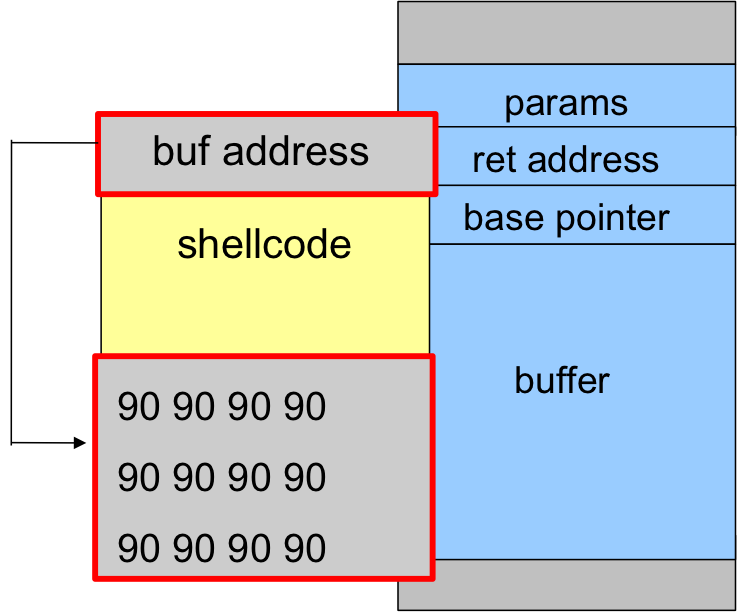
\includegraphics[width=0.7\textwidth]{images/nop-sledding.png}
	\end{center}
\end{frame}


\section{Exemple}
\subsection{Exploitation d'un buffer overflow}
\begin{frame}[fragile]{Code vulnérable}
	\definecolor{bg}{rgb}{0.95,0.95,0.95}
	\begin{minted}[mathescape,
               linenos,
               numbersep=5pt,
               frame=lines,
               framesep=2mm,
               bgcolor=bg,
               baselinestretch=0.3,
               fontize=\footnotesize]{c}
#include <stdio.h>
#include <stdlib.h>
#include <string.h>

int main(int argc, char *argv[]) {
    char buffer[256] = {0};

    if (argc < 2) {
        printf("Usage: %s username\n", argv[0]);
        exit(1);
    }

    /* strcpy is unsafe */
    strcpy(buffer, argv[1]);
    printf("Your username is: %s\n", buffer);

    return 0;
}
	\end{minted}
\end{frame}

\begin{frame}{Problèmes}
	\begin{itemize}
		\itemsep1.3em
		\item Pas de contrôle sur l'input de la part du programmeur
		\item Taille fixe des buffers
		\item Utilisation de strcpy
		\begin{itemize}
			\itemsep1.3em
			\item[] "BUGS\\
       If the destination string of a strcpy() is not large enough, then\\
       \textbf{anything}  might  happen." (Source: man strcpy)
		\end{itemize}
		\item[] $\Rightarrow$ \Large{Présence d'un buffer overflow !}
	\end{itemize}
\end{frame}

\begin{frame}{Demo}
	\begin{center}
		\Huge{DEMO} \\
		\Large{Exploitation d'un buffer overflow (sans protection)}
	\end{center}
\end{frame}

\section{Questions}

\begin{frame}{Questions ?}
	\begin{center}
		
\includegraphics[height=3cm,width=3cm]{images/LogoHackGyver.png} \\
		\Huge{Questions ?}
	\end{center}
\end{frame}

\end{document}
